\newpage\section*{Worksheet 7, \Course, \Semester} 
\noindent \Sections 3.7, 3.8, 3.9

\subsection*{Exercises}

\begin{enumerate}
	\item Differentiate the following functions. 
    \begin{enumerate}
    	\item $\displaystyle v(t) = 2^{3t}$
    	\item $\displaystyle y(x) = {\large x^{x^{x}}}, \quad x > 0$
        \item $\displaystyle u(x) = \sin\left(\tan^{-1} (\ln x)\right)$
        
        \item $\displaystyle s(t) = \log_2\left(\log_3\left(e^{t^2}\right)\right)$
        \item $\displaystyle a(t) = \ln\left(\frac{(t+2)^3(t+5)^7}{\sqrt{t-5}}\right)$
    \end{enumerate}
    \item The curve below is specified by the equation $$2\left(x^2+y^2\right)^2=25\left(x^2-y^2\right)$$
    
    \begin{center}
		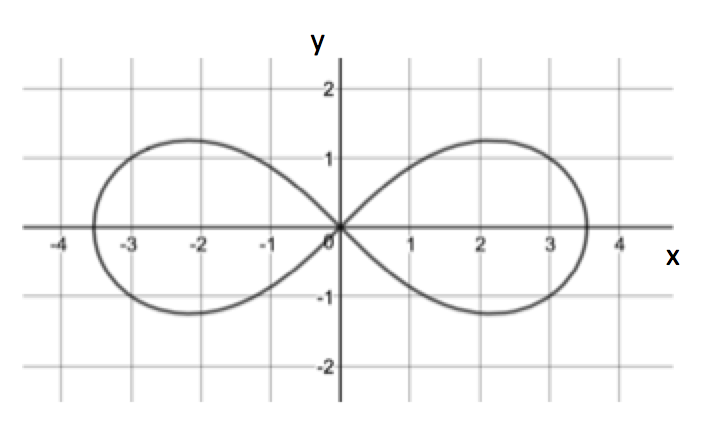
\includegraphics[width=0.7\textwidth]{images/imgWS7Implicit.png} 
    \end{center}
    
    
    
    
    \begin{enumerate}
    	\item By inspection, is the slope of the tangent line at $(3,1)$ positive, negative, or zero? 
        \item Construct the equations of the tangent line, and the normal line, at the point $(3,1)$. 
\end{enumerate}
\end{enumerate}